\documentclass[UTF8,linespread=1.236]{ctexart}
\usepackage{subfig}
\usepackage{listings}
\usepackage{amsmath}
\usepackage{booktabs}
\usepackage[a4paper,centering,top=3cm,left=2.6cm]{geometry}

\pagestyle{plain}
\ctexset {
    section = {
        name = {},
        number = {},
        aftername = {},
    },
    subsection = {
        name = {,、},
        number = \chinese{subsection},
        aftername = {},
    },
    subsubsection = {
        name = {},
        number = \arabic{subsubsection},
    }
}
\newcommand\unitV{\:\mathrm{V}}
\newcommand\unitOhm{\:\Omega}
\newcommand\pureunitA{\mathrm{A}}
\newcommand\pureunitV{\mathrm{V}}
\begin{document}

\title{电子技术基础实验报告}
\author{微电子与固体电子学院\ \ 傅宣登 (2016030102010)}

\maketitle
%\thispagestyle{empty}

\section{实验名称:叠加定理的验证}

\subsection{实验目的}

\begin{enumerate}
    \item 学习和掌握使用 Ngspice 进行电路仿真的方法。
    \item 掌握 Ngspice 中直流电压和直流电流的测试方法。
    \item 进一步加深对叠加定理的理解。
\end{enumerate}

\subsection{实验原理与测量方法}

\subsubsection{叠加定理}

叠加定理指出,全部电源在线性电路中产生的任一电压或电流,
等于每一个电源单独作用产生的相应电压或电流的代数和。

考虑如图 \ref{circuits-sub-a} 所示的电路,
电路中各支路电流、电压等于图 \ref{circuits-sub-b} 中 $u_{1S}$ 单独作用产生的电流、电压
与图 \ref{circuits-sub-c} 中 $u_{2S}$ 单独作用产生的电流、电压的代数和。

\begin{figure}[htbp]
\centering
\subfloat[完整电路]{\label{circuits-sub-a}
\begin{minipage}{0.29\textwidth}
    \centering
    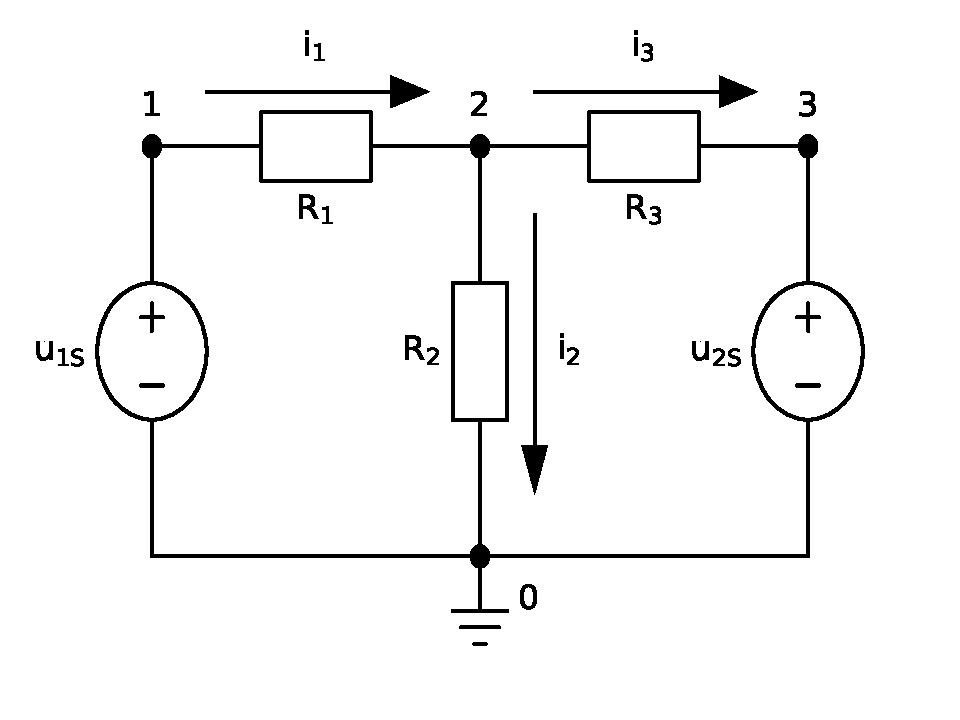
\includegraphics[width=\textwidth]{complete.pdf}
\end{minipage}}
\qquad
\subfloat[$u_{1S}$ 单独作用]{\label{circuits-sub-b}
\begin{minipage}{0.29\textwidth}
    \centering
    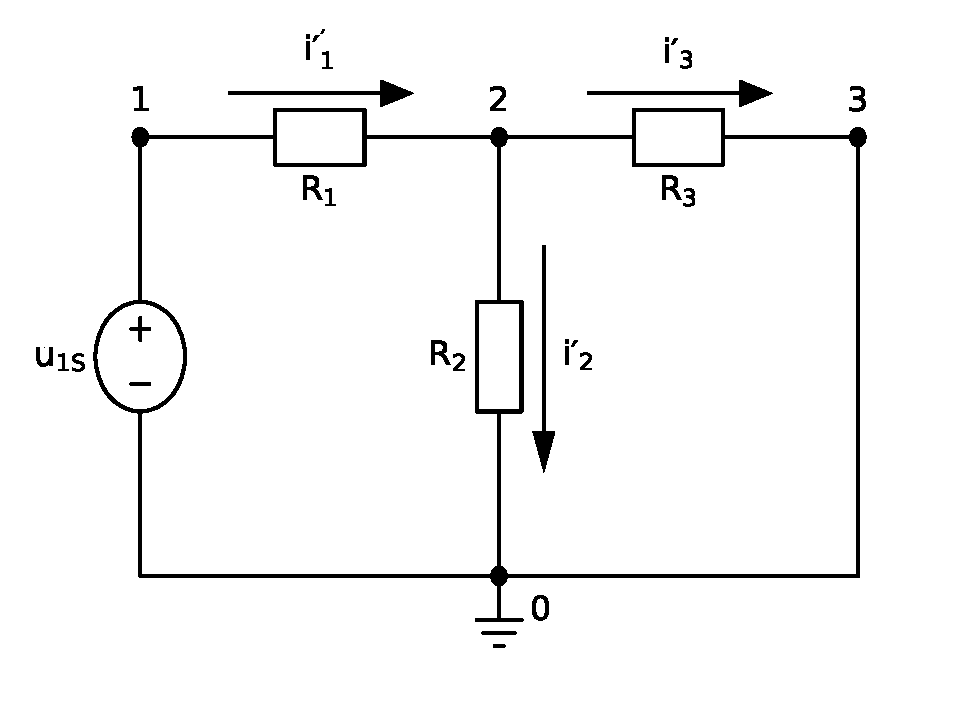
\includegraphics[width=\textwidth]{vs1.pdf}
\end{minipage}}
\qquad
\subfloat[$u_{2S}$ 单独作用]{\label{circuits-sub-c}
\begin{minipage}{0.29\textwidth}
    \centering
    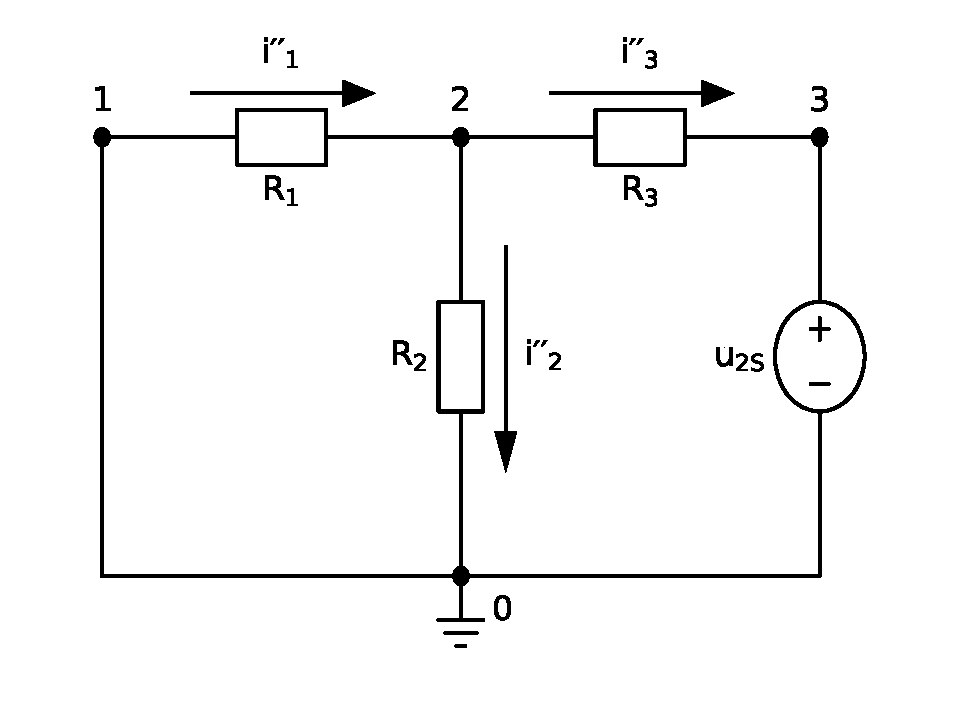
\includegraphics[width=\textwidth]{vs2.pdf}
\end{minipage}}
\caption{叠加定理原理图}\label{circuits}
\end{figure}

\subsubsection{测量方法}

Ngspice 与 Multisim 的核心都是 SPICE 引擎。
%与 Multisim 不同的是,Ngspice 是一款自由软件。
%为远离高昂的授权费用或获取免费教育版的周折,
本文使用自由软件 Ngspice 进行电路仿真。

在 Ngspice 中,电路是通过一种名为 \verb|netlist| 的文本文件描述的。

在图 \ref{circuits} 所示电路中,选取
\[
\begin{aligned}
u_{1S} &= 5 \unitV & u_{2S} &= 2 \unitV \\
R_1 &= 2 \unitOhm & R_2 &= 3 \unitOhm \quad R_3 = 4 \unitOhm
\end{aligned}
\]
则该电路可通过图 \ref{netlistfile} 所示的 \verb|netlist| 来描述。
其中 \verb|va| 是一个 $0\unitV$ 的电压源,
用来充当电流表以方便测定 $R_2$ 所在支路的电流。

\begin{figure}[!htbp]
\centering
\fbox{\begin{minipage}[c]{0.8\textwidth}
*** complete.cir *** \\
.title Verification of the superposition theorem - Complete Circuit. \\

vs1 1 0 dc 5 \\
vs2 3 0 dc 2 \\
r1 1 2 2 \\
r2 2 4 3 \\
r3 2 3 4 \\

va 4 0 dc 0 ; Ammeter to measure current into R2

.end
\end{minipage}}
\caption{完整电路的 netlist}\label{netlistfile}
\end{figure}

将其中 \verb|vs1| 或 \verb|vs2| 的电压改为 $0$ 即可描述某个电压源单独作用时的分电路。
将上述 \verb|netlist| 文件分别存为 \verb|complete.cir|、\verb|vs1.cir|、\verb|vs2.cir|。

当 \verb|netlist| 文件准备好后,就在终端下运行下面的命令进入 Ngspice 了。
\begin{lstlisting}{language=bash}
$ ngspice
\end{lstlisting}

进入 Ngspice 环境后,运行以下命令载入指定电路并准备仿真数据的读取,
\begin{lstlisting}{language=bash}
-> source netlist.cir
-> op
\end{lstlisting}

这时可以通过 \verb|print| 命令获取电路响应信息了。
\begin{lstlisting}{language=bash}
-> print -i(vs1),i(va),i(vs2)
-> print v(1,2),v(2),v(2,3)
\end{lstlisting}
上述代码显示了载入的电路各节点电压和支路电流。

\subsection{实验内容}

运行 Ngspice 并载入电路文件、模拟仿真后,记录相关数据于表 \ref{tab:expdata} 中。
\begin{table}[htb]
\centering
\begin{tabular}{ccccccc}
\toprule
参数 & $I_{R1}/\pureunitA$ & $I_{R2}/\pureunitA$ & $I_{R3}/\pureunitA$ & $U_{R1}/\pureunitV$ & $U_{R2}/\pureunitV$ & $U_{R3}/\pureunitV$ \\
\midrule
$U_{S1}$ 单独作用 & $1.35$ & $0.77$ & $0.58$ & $2.69$ & $2.31$ & $2.31$ \\
$U_{S2}$ 单独作用 & $-0.23$ & $0.15$ & $-0.38$ & $-0.46$ & $0.46$ & $-1.54$ \\
共同作用时的测量值 & $1.12$ & $0.92$ & $0.19$ & $2.23$ & $2.77$ & $0.77$ \\
\bottomrule
\end{tabular}
\caption{仿真实验数据}\label{tab:expdata}
\end{table}

\clearpage

\subsection{数据分析与结论}

分析上表数据可知,在误差范围内,
线性电路中各支路电流、电压等于 $U_{S1}$ 与 $U_{S2}$ 单独作用产生的电流、电压的代数和。叠加定理是正确的。

\end{document}
